
\begin{figure}
	\centering
	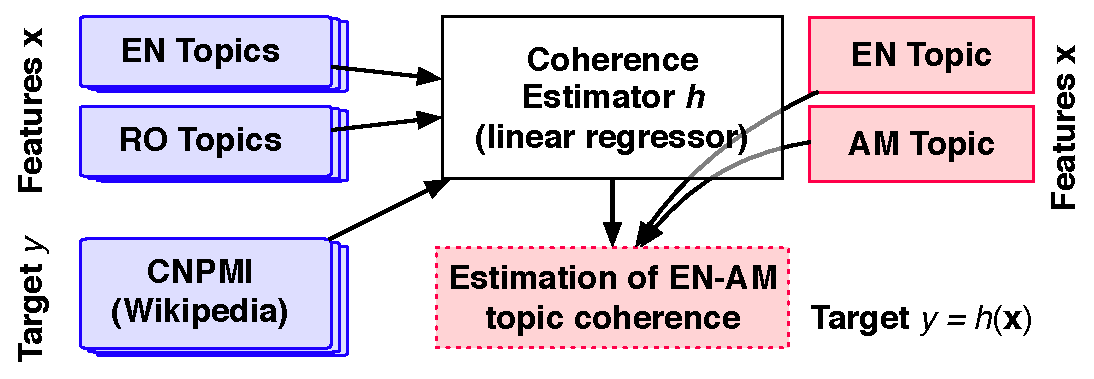
\includegraphics[width=\linewidth]{2018_naacl_mltm_eval/figures/calibrator}
	\caption{The coherence estimator takes multilingual topics and
          features from them then outputs an estimated topic coherence.}
	\label{fig:calibrator}
\end{figure}

\section{Adapting to Low-Resource Languages}
\label{sec:coherence-estimator}







\cnpmi{} needs a reference corpus for co-occurrence statistics.
Wikipedia, which has good coverage of topics and vocabularies is a
common choice~\cite{JHL16}.  Unfortunately, Wikipedia is often
unavailable or not large enough for low-resource languages. It only
covers $282$
languages,\footnote{\smallurl{https://meta.wikimedia.org/wiki/List_of_Wikipedias}}
and only $249$ languages have more than $1{,}000$ pages: many of pages
are short or unlinked to a high-resource language. Since \cnpmi{}
requires comparable documents, the usable reference corpus is
defined by \emph{paired} documents.

Another option for a parallel reference corpus is the Bible~\cite{resnik-99}, which
is available in most world languages;\footnote{The Bible
  is available in $2{,}530$ languages.} however, it is small
and archaic. It is good at evaluating topics such as
\underline{family} and \underline{religion}, but not ``modern'' topics
like \underline{biology} and \underline{Internet}.  Without reference
co-occurrence statistics relevant to these topics, \cnpmi{} will fail
to judge topic coherence---it must give the ambiguous answer of zero.
Such a score could mean a totally incoherent topic where each word
pair never appears together (Topics~6 in Figure~\ref{fig:example}), or
an unjudgeable topic (Topic~5).


\begin{figure*}[t!]
  \newcommand{\estimatorl}{.3}
  \newcommand{\estimatorr}{.65}
\begin{tabular}{cl}
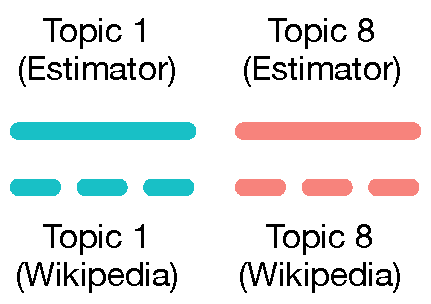
\includegraphics[width=.2\linewidth]{2018_naacl_mltm_eval/figures/estimator_legend}&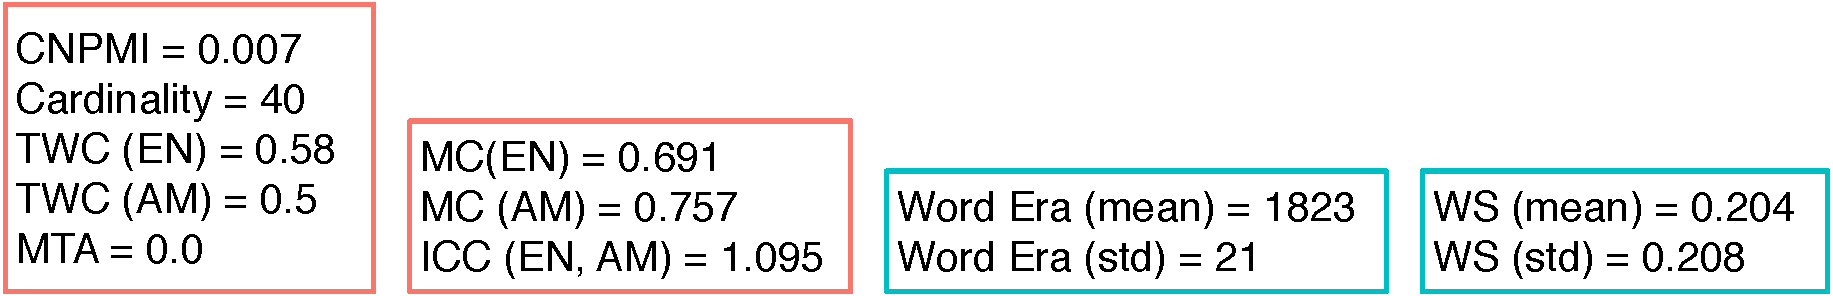
\includegraphics[width=\estimatorr\linewidth]{2018_naacl_mltm_eval/figures/estimator_top_features}\\
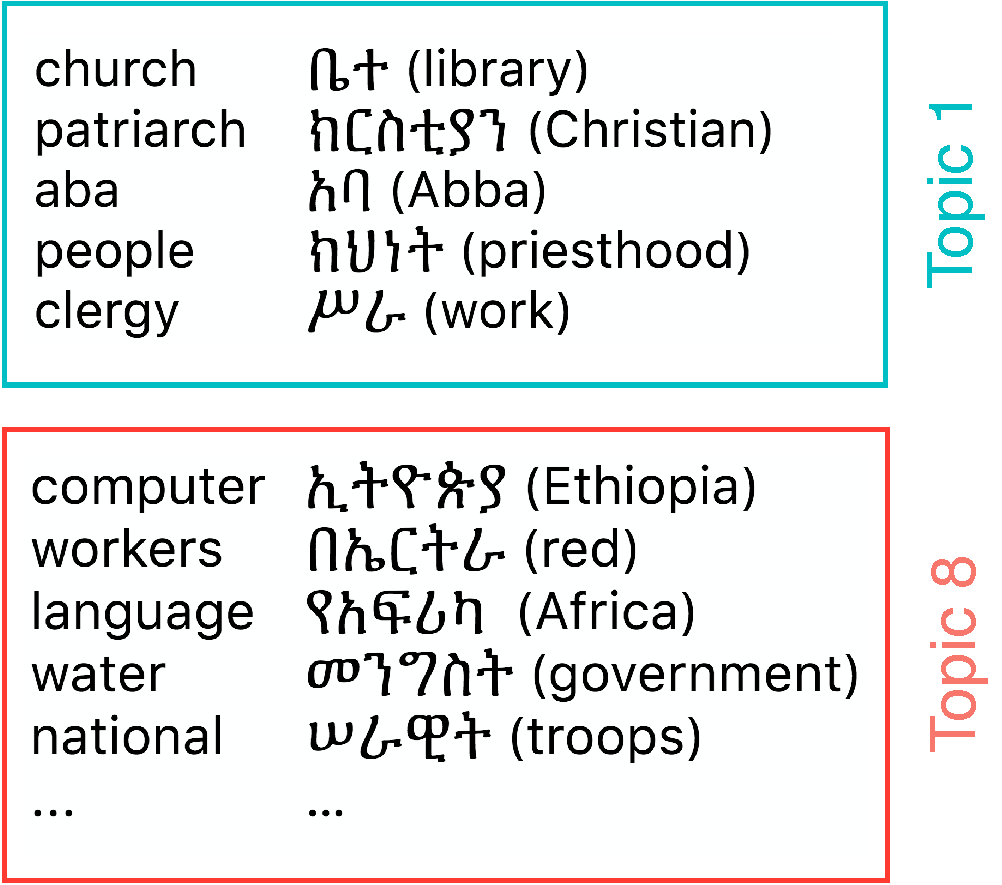
\includegraphics[width=\estimatorl\linewidth]{2018_naacl_mltm_eval/figures/estimator_topics}&\includegraphics[width=\estimatorr\linewidth]{2018_naacl_mltm_eval/auto_fig/estimator_example}\\
& 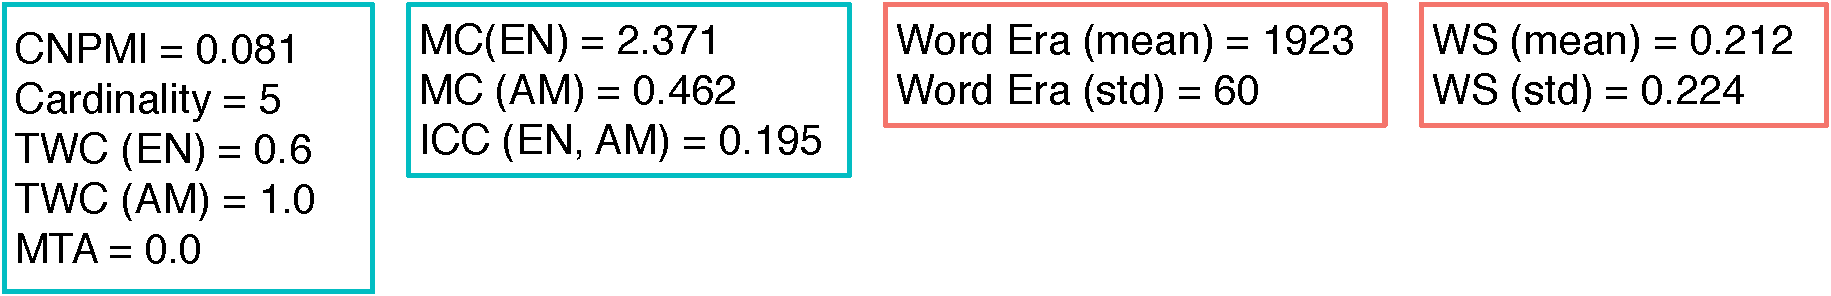
\includegraphics[width=\estimatorr\linewidth]{2018_naacl_mltm_eval/figures/estimator_bottom_features}
\end{tabular}
	\caption{As the estimator adds additional features, the
          estimated topic coherence scores (solid lines) approach to
          Wikipedia \cnpmi{} (dashed lines).}
	\label{fig:example2}
\end{figure*}



Our goal is to obtain a reliable estimation of topic coherence for
low-resource languages when the Bible is the only reference.  We
propose a model that can correct the drawbacks of a Bible-derived
\cnpmi{}.  While we assume bilingual topics paired with
English, our approach can be applied to any high-resource/low-resource
language pair.




We take Wikipedia's \cnpmi{} from high-resource languages as accurate
estimations.  We then build a coherence
\textit{estimator} 
on topics from high-resource languages, with the Wikipedia \cnpmi{} as
the target output.  We use linear regression using the below features.
Given a topic in low-resource language, the estimator produces an
estimated coherence (Figure~\ref{fig:calibrator}).


\subsection{Estimator Features}

The key to the estimator is to find features that capture whether
we should trust the Bible.
For generality, we focus on features independent
of the available resources other than the Bible.
This section describes the features, which we split into four groups.

\paragraph{Base Features (\textsc{base})}
Our base features include information we can collect from
the Bible and the topic model:
cardinality $C$, \cnpmi{} and \inpmi{}, \mta{}, and topic word coverage (\textsc{twc}),
which counts the percentage of topic words in a topic that appear in a reference corpus.

\paragraph{Crosslingual Gap (\textsc{gap})}

A low \cnpmi{} score could indicate a topic pair where each language has
a monolingually coherent topic but that are not about the same theme
(Topic 6 in Figure~\ref{fig:example}). Thus, we add two features to
capture this information using the Bible: mismatch coefficients (\mc{}) and
internal comparison coefficients (\icc{}):
\begin{align}
\mc{}({\ell_1 ; \ell_2,k}) &= \frac{\cnpmi{}(\ell_1,\ell_2,k)}{\inpmi{}(\ell_1,k) + \alpha},\\
\icc{}(\ell_1,\ell_2,k) &= \frac{\inpmi{}(\ell_1,k) + \alpha}{\inpmi{}(\ell_2,k) + \alpha},
\end{align}
where $\alpha$ is a smoothing factor ($\alpha=0.001$ in our
experiments). \mc{} recognizes the gap between crosslingual and monolingual coherence,
so a higher \mc{} score indicates a gap between coherence within and across languages.
Similarly, \icc{} compares monolingual coherence to tell if both languages are coherent:
the closer to $1$ the \icc{} is,
the more comparable internal coherence both languages have.

\paragraph{Word Era (\textsc{era})}

Because the Bible's vocabulary is unable to evaluate modern topics, we
must tell the model what the modern words are.  The \textbf{word era}
features are the earliest usage year
\footnote{\smallurl{https://oxforddictionaries.com/}} for each word in
a topic.  We use both the mean and standard deviation as features.



\paragraph{Meaning Drift (\textsc{drift}).}

The meaning of a word can expand and drift over time.  For example, in the Bible,
``web'' appears in Isaiah~59:5:
\begin{displayquote}
	They hatch cockatrice' eggs, and weave the spider's \textbf{web}.
\end{displayquote}
The word ``web'' could be evaluated correctly in an \underline{animal}
topic. For modern topics, however, Bible fails to capture modern meanings of ``web'',
as in Topic~5 (Figure~\ref{fig:example}).

To address this \textbf{meaning drift}, we use a
method similar to \newcite{HamiltonLJ16}. For each English
word, we calculate the context vector from Bible and from Wikipedia
with a window size of five and calculate the cosine similarity between
them as \textbf{word similarity}.  Similar context vectors mean
that the usage in the Bible is consistent with Wikipedia.
We calculate word similarities for all the English topic words in a
topic and use the average and standard deviation as features.

\subsection{Example}


	
	



	

In Figure~\ref{fig:example2}, Topic~1 is coherent while Topic~8 is
not. From left to right, we incrementally add new feature sets, and
show how the estimated topic coherence scores (dashed lines) approach
the ideal \cnpmi{} (dotted lines). When only using the \textsc{base}
features, the estimator gives a higher prediction to Topic~8 than to
Topic~1. Their low \mta{} and \textsc{twc} prevent accurate
evaluations.  Adding \textsc{gap} does not help much.  However,
$\icc{}(\textsc{en},\textsc{am},k=1)$ is much smaller, which might
indicate a large gap of internal coherence between the two languages.

Adding \textsc{era} makes the estimated scores flip between the two
topics.  Topic~1 has word era of $1823$, much older than Topic 8's
word era of $1923$, indicating that Topic~8 includes modern words the
Bible lacks (\textit{e.g.}, ``computer'').  Using all the features,
the estimator gives more accurate topic coherence evaluations.
